%%%%%%%%%%%%%%%%%%%%%%%%%%%%%%%%%%%%%%%%%
% Classicthesis Typographic Thesis
% LaTeX Template
% Version 1.4 (1/1/16)
%
% This template has been downloaded from:
% http://www.LaTeXTemplates.com
%
% Original author:
% André Miede (http://www.miede.de) with commenting modifications by:
% Vel (vel@LaTeXTemplates.com)
%
% License:
% GNU General Public License (v2)
%
% General Tips:
% 1) Make sure to edit the classicthesis-config.file
% 2) New enumeration (A., B., C., etc in small caps): \begin{aenumerate} \end{aenumerate}
% 3) For margin notes: \marginpar or \graffito{}
% 4) Do not use bold fonts in this style, it is designed around them
% 5) Use tables as in the examples
% 6) See classicthesis-preamble.sty for useful commands
%
%%%%%%%%%%%%%%%%%%%%%%%%%%%%%%%%%%%%%%%%%

%----------------------------------------------------------------------------------------
%	SILENCE ANNOYING WARNINGS
%----------------------------------------------------------------------------------------

\RequirePackage{silence}
\WarningFilter{titlesec}{Non standard sectioning command}
\WarningFilter{scrreprt}{Usage of package}
\WarningFilter{scrreprt}{Activating an ugly workaround}
\WarningFilter{titlesec}{Non standard sectioning command detected}


% **************************************************
% Document Class Definition
% **************************************************
\documentclass[%
	paper=A4,					% paper size --> A4 is default in Germany
	twoside=true,				% onesite or twoside printing
	openright,					% doublepage cleaning ends up right side
	parskip=full,				% spacing value / method for paragraphs
	chapterprefix=true,			% prefix for chapter marks
	11pt,						% font size
	headings=normal,			% size of headings
	bibliography=totoc,			% include bib in toc
	listof=totoc,				% include listof entries in toc
	titlepage=on,				% own page for each title page
	captions=tableabove,		% display table captions above the float env
	draft=false,				% value for draft version
    openany						% Avoid blank page after each new part, chapter, ...
]{scrreprt}%

%%%%%%%%%%%%%%%%%%%%%%%%%%%%%%%%%%%%%%%%%
% Thesis Configuration File
%
% This file has been downloaded from:
% http://www.LaTeXTemplates.com
%
% Original author:
% André Miede (http://www.miede.de) with extensive commenting changes by:
% Vel (vel@LaTeXTemplates.com)
%
% License:
% GNU General Public License (v2)
%
% Important note:
% The main lines to change in this file are in the DOCUMENT VARIABLES
% section, the rest of the file is for advanced configuration.
%
%%%%%%%%%%%%%%%%%%%%%%%%%%%%%%%%%%%%%%%%%

\usepackage[utf8]{inputenc}		% defines file's character encoding

\usepackage[french,main=french]{babel} % babel system, adjust the language of the content

\usepackage[					% clean thesis style
	figuresep=colon,%
	sansserif=true,%
	hangfigurecaption=false,%
	hangsection=true,%
	hangsubsection=true,%
	colorize=full,%
	colortheme=bluegreen,%
% LLT: Use biber if using UTF8 encoding
% 	bibsys=bibtex,%
	bibsys=biber,%
% 	bibfile=bib-refs,%
    bibfile=library,%
	bibstyle=numeric,%
%     bibstyle=apa,%
]{cleanthesis}

% **************************************************
% DOCUMENT VARIABLES
% **************************************************
% \newcommand{\thesisTitle}{D\'eveloppement de nouvelles strat\'egies de pr\' ediction structurale à partir de contacts \'evolutifs\xspace}
\newcommand{\thesisTitle}{Comment la protéine prion PrP\up C est impliquée dans l'inflammation pulmonaire chronique?\\ Rôle de l'homéostasie du cuivre et du stress oxydatif\xspace}
\newcommand{\thesisName}{Amal Kouadri\xspace}
\newcommand{\thesisSubject}{Thèse de doctorat en Sciences de la Vie\xspace}
\newcommand{\thesisDate}{Automne 2017}
\newcommand{\thesisVersion}{0.1}

\newcommand{\thesisFirstReviewer}{Jane Doe}
\newcommand{\thesisFirstReviewerUniversity}{\protect{Clean Thesis Style University}}
\newcommand{\thesisFirstReviewerDepartment}{Department of Clean Thesis Style}

\newcommand{\thesisSecondReviewer}{John Doe}
\newcommand{\thesisSecondReviewerUniversity}{\protect{Clean Thesis Style University}}
\newcommand{\thesisSecondReviewerDepartment}{Department of Clean Thesis Style}

\newcommand{\thesisFirstSupervisor}{Dr. Mohamed BENHAROUGA}
\newcommand{\thesisSecondSupervisor}{}

\newcommand{\thesisUniversity}{\protect{Université Grenoble Alpes}}
\newcommand{\thesisUniversityDepartment}{\'Ecole doctorale Chimie et Sciences du vivant}
\newcommand{\thesisUniversityInstitute}{CEA Grenoble}
\newcommand{\thesisUniversityGroup}{Laboratoire de Chimie et Biologie des Métaux (LCBM)\\ \'Equipe Biologie des Métaux (BioMet)}
\newcommand{\thesisUniversityCity}{Grenoble}
\newcommand{\thesisUniversityStreetAddress}{17 rue des martyrs}
\newcommand{\thesisUniversityPostalCode}{38000}

%----------------------------------------------------------------------------------------
%	USEFUL COMMANDS
%----------------------------------------------------------------------------------------

\newcommand{\ie}{i.\,e.}
\newcommand{\Ie}{I.\,e.}
\newcommand{\eg}{e.\,g.}
\newcommand{\Eg}{E.\,g.} 

\newcounter{dummy} % Necessary for correct hyperlinks (to index, bib, etc.)
\providecommand{\mLyX}{L\kern-.1667em\lower.25em\hbox{Y}\kern-.125emX\@}
\newlength{\abcd} % for ab..z string length calculation

% **************************************************
% Load and Configure Packages
% **************************************************

\hypersetup{					% setup the hyperref-package options
	pdftitle={\thesisTitle},	% 	- title (PDF meta)
	pdfsubject={\thesisSubject},% 	- subject (PDF meta)
	pdfauthor={\thesisName},	% 	- author (PDF meta)
	plainpages=false,			% 	-
	colorlinks=true,			% 	- colorize links?
    linktocpage=true,
	pdfborder={0 0 0},			% 	-
	breaklinks=true,			% 	- allow line break inside links
	bookmarksnumbered=true,		%
	bookmarksopen=true,			%,
    linkcolor=ctcolorblue,
    citecolor=black,
}

\PassOptionsToPackage{acronym,translate=babel,xindy,toc,nopostdot,nonumberlist}{glossaries}
\usepackage{glossaries}

\usepackage{chngcntr}			% Reset Chapter counter for each part
\counterwithin*{chapter}{part}

\DeclareCiteCommand{\citeauthorfirstlast}
  {\boolfalse{citetracker}%
   \boolfalse{pagetracker}%
   \DeclareNameAlias{labelname}{first-last}%
   \usebibmacro{prenote}}
  {\ifciteindex
     {\indexnames{labelname}}
     {}%
   \printnames{labelname}}
  {\multicitedelim}
  {\usebibmacro{postnote}}


% **************************************************
% Debug LaTeX Information
% **************************************************
%\listfiles
%----------------------------------------------------------------------------------------
%	Glossary
%----------------------------------------------------------------------------------------
\newglossaryentry{recuit}{
    name={recuit simulé},
    description={Protocole de recherche de la forme la plus stable du système étudié. Cette forme est dans ce casElle de plus basse énergie correspondant à la recherche du minimum global de la surface d'énergie potentielle du système moléculaire. Cette méthode a une phase de simulation à haute température permettant d'explorer l'espace conformationnel et une deuxième de refroidissement pour atteindre un autre minimum local ou global du système.}
}
\newglossaryentry{coupscal}{
    name={couplage scalaire},
    description={Interaction correspondant à un transfert d'aimantation entre deux noyaux séparés par une ou plusieurs liaisons covalentes. La force est mesurée par les constantes de couplage qui dépendent du type des noyaux impliqués.}
}
\newglossaryentry{coupdip}{
    name={couplage dipolaire},
    description={Association entre deux noyaux proches dans l'espace. Le transfert d'aimantation observés entre les deux noyaux est affecté par les mouvements browniens en solution. Cet effet est communément nommé  dans cette situation l'effet Overhauser nucléaire (\acrshort{noe}).},
    plural={couplages dipolaires}
}
\newglossaryentry{cdr}{
    name={contrainte de distance ambiguë},
    description={Chaque pic croisé d'un spectre \acrshort{noesy} est traité comme étant la superposition des signaux  des assignations possibles du pic. Les contraintes calculées (Distance effective $R$) sont proportionnelles à la somme de l'inverse des distances interatomiques élevées ($r$) à la puissance 6 de chaque assignation possible. \begin{equation}\frac{1}{R^6} = \sum_{i}^{n}\frac{1}{r_{i}^6}\end{equation}}
}
\newglossaryentry{rdc}{
    name={couplage dipolaire résiduel},
    description={Dans le cas d'expérimentations \acrshortpl{rmn} dans des milieux partiellements orientés, des couplages dipolaires résiduels sont mesurés et leur valeur est proportionnelle à $\frac{1}{r^3}$ ($r$ est la distance inter-atomique) mais dépend également des angles $\theta$ entre les liaisons covalentes et le vecteur du champ magnétique statique. }
}
\newglossaryentry{apidef}{
    name={interface de programmation (API)},
    description={Regroupe l'ensemble des classes, méthodes et fonctions d'une application souvent stockés dans une bibliothèque logicielle et qui permettent aux autres logiciels d'avoir accès aux différentes fonctionnalités de l'application. Elle correspond par exemple aux classes d'ARIA sauvegardant les paramètres.}
}
\newglossaryentry{framew}{
    name={framework},
    description={Ensemble cohérent de composants logiciels permettant de définir les bases d'une application. Il définit un environnement de travail au développeur proposant un ensemble d'outils et guide l'architecture du futur logiciel.}
}
\newglossaryentry{ormdef}{
    name={mapping objet relationnel (ORM)},
    description={Concept de programmation permettant de convertir un ensemble d'objets en une base de données relationnelle.}
}

%----------------------------------------------------------------------------------------
%	Acronyms
%----------------------------------------------------------------------------------------
\newacronym{xml}{XML}{Extensible Markup Language}
\newacronym{noesy}{NOESY}{Spectroscopie d'Effet Overhauser Nucleaire}
\newacronym{aria}{ARIA}{Ambiguous Restraints for Iterative Assignment}
\newacronym{rmn}{RMN}{Résonance Magnétique Nucléaire}
\newacronym{cns}{CNS}{Crystallography \& NMR System}
\newacronym{mtf}{MTF}{Molecular Topology File}
\newacronym{noe}{NOE}{Effet Overhauser Nucléaire}
\newacronym{embl}{EMBL}{European Molecular Biology Laboratory}
\newacronym{bis}{BIS}{Bioinformatique Structurale}
\newacronym{wenmr}{WeNMR}{Worldwide e-Infrastructure for NMR and structural biology}
\newacronym{api}{API}{Interface de Programmation (Application Programming Interface)}
\newacronym{cib}{CIB}{Centre d'Informatique pour la Biologie}
\newacronym{ccpn}{CCPN}{Collaborative Computing Project for the NMR community}
\newacronym{pdb}{PDB}{Protein Data Bank}
\newacronym{mtv}{MTV}{Modèle Template Vue}
\newacronym{mvc}{MVC}{Modèle Vue Contrôleur}
\newacronym{html}{HTML}{Hypertext Markup Language}
\newacronym{orm}{ORM}{Mapping Objet Relationnel}
\newacronym{rmsd}{RMSD}{Root Mean Square Deviation}
\newacronym{dry}{DRY}{Don't Repeat Yourself}
\newacronym{cgi}{CGI}{Common Gateway Interface}
\newacronym{casd}{CASD-NMR}{Critical Assessment of Automated Structure Determination of Proteins from NMR Data}
\makeglossaries

% **************************************************
% Document CONTENT
% **************************************************
\begin{document}

%----------------------------------------------------------------------------------------
%	PRE-CONTENT THESIS PAGES
%----------------------------------------------------------------------------------------

% \frenchspacing % Reduces space after periods to make text more compact

% \raggedbottom % Makes all pages the height of the text on that page

\pagenumbering{roman} % Roman page numbering prior to the start of the thesis content (i, ii, iii, etc)
\pagestyle{empty} % Suppress headers for the pre-content pages

% !TEX root = ../thesis-example.tex
%
% ------------------------------------  --> cover title page
\begin{titlepage}
	\pdfbookmark[0]{Cover}{Cover}
	\flushright
	\hfill
	\vfill
	{\LARGE\thesisTitle \par}
	\rule[5pt]{\textwidth}{.4pt} \par
	{\Large\thesisName}
	\vfill
	\textit{\large\thesisDate} \\
	Version: \thesisVersion
\end{titlepage}


% ------------------------------------  --> main title page
\begin{titlepage}
	\pdfbookmark[0]{Titlepage}{Titlepage}
	\tgherosfont
	\centering

	{\Huge \thesisUniversity} \\[2mm]
    {\Large \thesisUniversityDepartment} \\[4mm]
	
\includegraphics[width=6cm]{gfx/logo-uga.png} \\[2mm]
	
	\textsf{\large \thesisUniversityGroup} \\
    \textsf{\large \thesisUniversityInstitute} \\

	\vfill
	{\Large \thesisSubject} \\[5mm]
	{\LARGE \color{ctcolortitle}\textbf{\thesisTitle} \\[10mm]}
	{\Large \thesisName} \\

	\vfill
	\begin{minipage}[t]{.27\textwidth}
		\raggedleft
		\textit{1. Reviewer}
	\end{minipage}
	\hspace*{15pt}
	\begin{minipage}[t]{.65\textwidth}
		{\Large \thesisFirstReviewer} \\
	  	{\small \thesisFirstReviewerDepartment} \\[-1mm]
		{\small \thesisFirstReviewerUniversity}
	\end{minipage} \\[5mm]
	\begin{minipage}[t]{.27\textwidth}
		\raggedleft
		\textit{2. Reviewer}
	\end{minipage}
	\hspace*{15pt}
	\begin{minipage}[t]{.65\textwidth}
		{\Large \thesisSecondReviewer} \\
	  	{\small \thesisSecondReviewerDepartment} \\[-1mm]
		{\small \thesisSecondReviewerUniversity}
	\end{minipage} \\[10mm]
	\begin{minipage}[t]{.27\textwidth}
		\raggedleft
		\textit{Encadrants}
	\end{minipage}
	\hspace*{15pt}
	\begin{minipage}[t]{.65\textwidth}
		\thesisFirstSupervisor\ et \thesisSecondSupervisor
	\end{minipage} \\[10mm]

	\thesisDate \\
    \vfill
    


\end{titlepage}


% ------------------------------------  --> lower title back for single page layout
\hfill
\vfill
{
	\small
	\textit{\thesisTitle,} \thesisName \\
    \textcopyright\ \thesisDate \\
	\thesisSubject\\
	Rapporteurs: \thesisFirstReviewer\ and \thesisSecondReviewer \\
	Directeur de th\`ese: \thesisFirstSupervisor\\
	\textbf{\thesisUniversity} \\
	\thesisUniversityDepartment \\
    \textit{\thesisUniversityGroup} \\
	\thesisUniversityInstitute \\
	\thesisUniversityStreetAddress \\
	\thesisUniversityPostalCode\ \thesisUniversityCity
}
		% INCLUDE: all titlepages

\pagestyle{plain}				% display just page numbers

\clearpage% !TEX root = ../thesis-example.tex
%
\pdfbookmark[0]{\abstractname}{\abstractname}

\begingroup

\let\clearpage\relax
\let\cleardoublepage\relax
\let\cleardoublepage\relax

\chapter*{\abstractname}\label{sec:abstract}
\vspace*{-10mm}

Dans la fibrose kystique (FC), l'inflammation est détectée au début de la voie aérienne, même avant le début de l'infection bactérienne. Cela suggère que les mécanismes autres que l'infection sont à l'origine du processus initial d'inflammation. Parmi ces processus, il y a le stress oxydatif. Ce dernier est largement reconnu comme un élément essentiel de plusieurs maladies.
Récemment, nous avons observé que les cellules et les tissus des patients bronchiques des FC présentent une augmentation de la concentration de Cu, dans la production de radicaux libres, dans les activités enzymatiques pro et antioxydantes, et une diminution de la concentration de glutathion, un chelate naturel de Cu intracellulaire. Ces résultats et d'autres nous ont permis d'établir le lien avec Cu, le stress oxydatif, l'inflammation et l'infection.
En étudiant le niveau d'expression d'un certain nombre de gènes codant pour les protéines de l'homéostasie du Cu, nous avons constaté que l'expression de la protéine prion cellulaire (PrPC) a été modifiée. PrPC est une glycoprotéine chantée de glycosyl phosphatidyl inositol (GPI) qui a été impliquée dans la propagation et l'agrégation des prions dans le système nerveux central qui conduit à des maladies des encéphalopathies spongiformes transmissibles (EST).
Cependant, en dépit de plusieurs études in vitro et in vivo qui ont démontré la capacité de PrPC à interagir avec d'autres protéines, à lier le cuivre (Cu) avec une affinité élevée et à protéger les cellules contre le stress oxydatif, ses fonctions physiologiques sont encore à l'étude, en particulier dans Des tissus extra-neuronaux, tels que l'épithélium bronchique.
Dans le présent projet, nous avons étudié le rôle de PrPC dans l'architecture cellulaire pulmonaire en déterminant son impact sur l'intégrité des jonctions épithéliales pulmonaires par rapport à l'inflammation, l'homéostasie du Cu, le stress oxydatif et l'infection. Dans ce cas, je présenterai seulement les résultats de la première partie de mon projet concernant le rôle physiologique de PrPC dans les cellules épithéliales bronchiques normales. En utilisant la PCR quantitative et l'immunoblotting, nous avons démontré que l'ARNm de PrPC et la protéine PrPC mature sont exprimés dans des cellules bronchiques épithéliales humaines (HBE et A549). Nous avons également démontré par immunofluorescence que le PrPC est localisé dans les domaines apicaux et latéraux où il se localise localement avec des jonctions de protéines adhérentes et désmosomes. La localisation du domaine PrPC dépend du niveau de polarisation de la cellule. Ces données ont été confirmées par la co-immunoprécipitation montrant une interaction de la protéine PrPC avec une protéine de jonction adhérente désmosome. En outre, nous avons montré que le traitement au Cu augmente l'expression de PrPC aux niveaux de l'ARNm et de la protéine, confirmant son rôle dans la protection cellulaire contre le stress oxydatif généré sur l'excès de cuivre. Enfin, nous avons démontré que l'invalidation du gène PrPC dans les cellules HBE diminue la résistance trans-épithéliale (TER), un indicateur de la qualité de la barrière de jonction.
Dans l'ensemble, nos résultats soulignent l'importance de PrPC dans le contrôle du contact cellulaire à cellulaire dans les cellules épithéliales pulmonaires normales et suggèrent que sa déréglementation pourrait affecter la barrière de jonction dans des maladies telles que la fibrose kystique.

\vspace*{20mm}

\renewcommand{\abstractname}{Abstract}
{\usekomafont{chapter}\abstractname}\label{sec:abstract-diff} \\

In cystic fibrosis (CF), inflammation is detected early in the airways, even before the onset of bacterial infection. This suggests that mechanisms other than infection are at the origin of the initial inflammation process. Among these processes, there is the oxidative stress. The latter is widely accepted as a critical component of several diseases. 
Recently, we observed that both cells and tissues from bronchial CF patients display an increase in Cu concentration, in free radicals production, in pro-and antioxidant enzyme activities, and a decrease in glutathione concentration, a natural intracellular Cu chelator. These results and others have allowed us to establish the link with Cu, oxidative stress, inflammation and infection.
While investigating the expression level of a number of genes encoding proteins of Cu homeostasis, we found that the expression of the cellular prion protein (PrPC) was altered. PrPC is a glycosyl phosphatidyl inositol (GPI)-anchored glycoprotein that have been involved in prion infection propagation and aggregation in the central nervous system that leads to transmissible spongiforme encephalopathies (TSE) diseases. 
However, despite several in vitro and in vivo studies that demonstrated the capacity of PrPC to interact with other proteins, to bind copper (Cu) with high affinity, and to protect cells against oxidative stress, its physiological functions are still under investigations, particularly in extra-neuronal tissues, such as bronchial epithelium. 
In the present project, we investigated the role of PrPC in the lung cellular architecture, by determining its impact on the integrity of the lung epithelial junctions in relation to inflammation, Cu homeostasis, oxidative stress, and infection.
Herein, I’ll only present the results of the first part of my project regarding the physiological role of PrPC in normal bronchial epithelial cells. Using quantitative PCR and immunoblotting, we demonstrated that the PrPC mRNA and the mature PrPC protein are expressed in human epithelial bronchial cells (HBE and A549). We also demonstrated by immunofluorescence that the PrPC is localized at the apical and lateral domains where it co-localizes with adherent and desmosomes protein junctions. The PrPC domain localization is dependent on the level of cell polarization. These data were confirmed by the co-immunoprecipitation showing an interaction of the PrPC protein with a protein of adherent desmosome junction. Moreover, we showed that Cu treatment increases PrPC expression at the mRNA and protein levels, confirming its role in the cellular protection from oxidative stress generated upon copper excess. Finally, we demonstrated that the invalidation of PrPC gene in HBE cells decreases the trans-epithelial resistance (TER), an indicator of the quality of the junctional barrier. 
Overall, our results stress the importance of PrPC in the control of cell to cell contact in normal lung epithelial cells and suggest that its deregulation might affect junction barrier in diseases such as cystic fibrosis.


\endgroup

\vfill		% INCLUDE: the abstracts (english and german)

% \cleardoublepage\include{FrontBackMatter/Foreword} % Uncomment and create a Foreword.tex to include a foreword

\clearpage% !TEX root = ../thesis-example.tex
%
\pdfbookmark[0]{Remerciements}{Remerciements} % Bookmark name visible in a PDF viewer

\begingroup

\let\clearpage\relax
\let\cleardoublepage\relax
\let\cleardoublepage\relax

\chapter*{Remerciements}
\label{sec:remerciements}

% \cleanchapterquote{We have seen that computer programming is an art, because it applies accumulated knowledge to the world, because it requires skill and ingenuity, and especially because it produces objects of beauty.}{Donald E. Knuth}{{C}omputer {P}rogramming as an {A}rt}
% \cleanchapterquote{In the drama of life on a molecular scale, proteins are where the action is.}{Lesk, Arthur M.}{{I}ntroduction to {P}rotein {A}rchitecture}

% \vspace*{-10mm}

\noindent \Blindtext[1][1]
\gls{recuit} \acrshort{pdb}

\endgroup % INCLUDE: acknowledgement
% \cleardoublepage
\clearpage
\clearpage% Table of Contents - List of Tables/Figures/Listings and Acronyms

\refstepcounter{dummy}

\pdfbookmark[1]{\contentsname}{tableofcontents} % Bookmark name visible in a PDF viewer

\setcounter{tocdepth}{2} % Depth of sections to include in the table of contents - currently up to subsections

\setcounter{secnumdepth}{3} % Depth of sections to number in the text itself - currently up to subsubsections

\tableofcontents 

\clearpage

\begingroup 
\let\clearpage\relax
\let\cleardoublepage\relax
\let\cleardoublepage\relax

%----------------------------------------------------------------------------------------
%	List of Figures
%----------------------------------------------------------------------------------------

\refstepcounter{dummy}
%\addcontentsline{toc}{chapter}{\listfigurename} % Uncomment if you would like the list of figures to appear in the table of contents
% \pdfbookmark[1]{\listfigurename}{lof} % Bookmark name visible in a PDF viewer

\listoffigures

\vspace*{8ex}
\newpage

%----------------------------------------------------------------------------------------
%	List of Tables
%----------------------------------------------------------------------------------------

\refstepcounter{dummy}
%\addcontentsline{toc}{chapter}{\listtablename} % Uncomment if you would like the list of tables to appear in the table of contents
% \pdfbookmark[1]{\listtablename}{lot} % Bookmark name visible in a PDF viewer

\listoftables
        
\vspace*{8ex}
\newpage
    
%----------------------------------------------------------------------------------------
%	List of Listings
%---------------------------------------------------------------------------------------- 

% \refstepcounter{dummy}
%\addcontentsline{toc}{chapter}{\lstlistlistingname} % Uncomment if you would like the list of listings to appear in the table of contents
% \pdfbookmark[1]{\lstlistlistingname}{lol} % Bookmark name visible in a PDF viewer

% \lstlistoflistings 

% \vspace{8ex}
% \newpage
       
%----------------------------------------------------------------------------------------
%	Acronyms
%----------------------------------------------------------------------------------------

%\addcontentsline{toc}{chapter}{Acronyms} % Uncomment if you would like the acronyms to appear in the table of contents
% \pdfbookmark[1]{Acronyms}{acronyms} % Bookmark name visible in a PDF viewer

% \chapter*{Acronyms}

\newpage
\refstepcounter{dummy}

\setglossarystyle{list} 
\printglossary[type=\acronymtype,title={Abbr\'eviations}]

%----------------------------------------------------------------------------------------
%	Glossary
%----------------------------------------------------------------------------------------

% \newpage
% \refstepcounter{dummy}

% \setglossarystyle{altlist} 
% \printglossary[title={Glossaire}]

% 
                   
\endgroup % Contents, list of figures/tables/listings and acronyms

% \setcounter{tocdepth}{2}		% define depth of toc
% \tableofcontents				% display table of contents
% \cleardoublepage

% \cleardoublepage % Avoids problems with pdfbookmark

%----------------------------------------------------------------------------------------
%	THESIS CONTENT - CHAPTERS
%----------------------------------------------------------------------------------------

\pagenumbering{arabic}			% arabic page numbering
\setcounter{page}{1}			% set page counter. Manually start the page counter at an arbitrary value (for example if you wish to count the pre-content pages in the page count)
\pagestyle{maincontentstyle} 	% fancy header and footer

%------------------------------------------------
\ctparttext{
\cleanchapterquote{La respiration est le berceau du rythme}{\citeauthorfirstlast{}}{\citetitle{}}
\cleanchapterquote{Rainer Maria Rilke}{\citeauthorfirstlast{}}{\citetitle{}}

En effet, nous avons besoin d’air pour vivre. L’air est composé à 78\% d’azote, 21\% d’oxygène et 1\% de gaz rares, mais seul l’oxygène est indispensable à la vie. Pour fonctionner les cellules de l’organisme ont besoin d’énergie, cette énergie est le résultat d’une réaction chimique entre les aliments que nous mangeons (glucides) et l’oxygène contenu dans l’air que nous respirons. Sans lui l’organisme ne pourrait pas produire d’énergies et nos organes ne pourraient pas fonctionner. D’autant que la réaction chimique entre les glucides et l’oxygène contenue dans l’air que nous respirons produit du dioxyde de carbone que nous expulsons également en respirant. 
L’arbre respiratoire (ou appareil respiratoire) est constitué des voies aériennes supérieurs (nez, bouche, larynx), de la trachée et des poumons. La proportion de cellules et l’épaisseur des épithéliums des voies respiratoires varient du haut (riche en cellules caliciformes et pluristratifié) en bas (riche en cellules cylindrique et uni-stratifié) de l’arbre respiratoire. Cette transition se fait progressivement}

\part{Le systeme respiratoire} % First part of the thesis

% Chapter X

\chapter{Trachée} % Chapter title


\label{ch:01-01} % For referencing the chapter elsewhere, use \autoref{ch:name} 

%----------------------------------------------------------------------------------------

% \section{}

La trachée fait suite au larynx, c’est un cylindre de 10 à 12 cm de long et de 1 à 2 cm de diamètre qui se termine par bifurcation en deux bronches principales au niveau du médiastin. La paroi trachéale est formée de trois couches: 
\begin{itemize}
\item La muqueuse de type respiratoire, comporte un épithélium pseudo stratifié composé de cellules ciliées et renfermant des cellules caliciformes qui sécrète le mucus. Le chorion est riche en fibres élastique, en glandes mixtes, en tissu lymphoïde ou la vascularisation est abondante et riche en nerfs La muqueuse a pour rôle entre autre d’empêcher le collapsus de la paroi trachéale pendant la respiration mais aussi le réchauffement, l’humidification et la filtration de l’air respiré
\item La tunique fibrocartilagineuse est constituée d’anneaux cartilagineux dans sa partie antérieure et les bandes musculaires lisses en postérieur lui confèrent sa flexibilité
\item L’adventice un tissus conjonctif riche en vaisseaux et en nerfs.
\end{itemize}

\begin{figure}[h!]
    \begin{minipage}[b]{0.4\linewidth}
        \centering 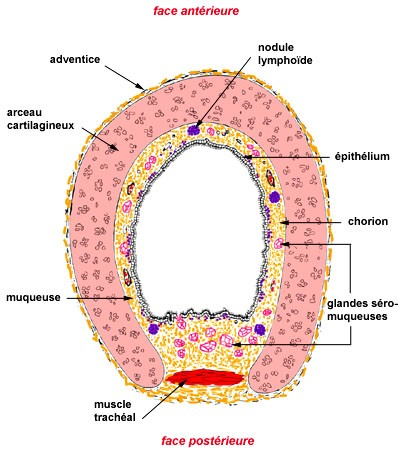
\includegraphics[scale=0.4]{gfx/Trach_esch_mas.jpg}
        \centering \caption{Schémas trachée}
        \label{Trachéeschémas}
    \end{minipage}\hfill
    \begin{minipage}[b]{0.7\linewidth}
        \centering 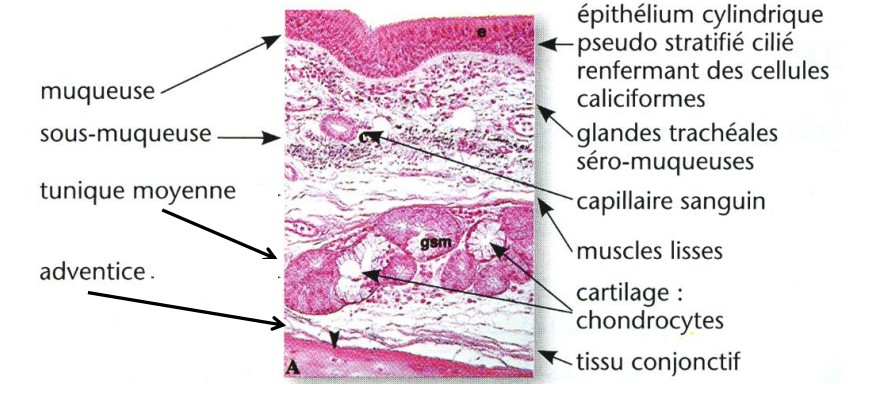
\includegraphics[scale=0.4]{gfx/Trach_ecoupe.jpg}
        \centering \caption{Coupe trachée}
        \label{Trachéecoupe}
    \end{minipage}
\end{figure}

La structure et la fonction de la trachée sont en relation étroite. De forme cylindrique elle assure le passage de l'air durant tout le cycle de la respiration, elle présente aussi, en relation avec son appareil mucociliaire, une fonction de drainage permettant l'élimination des particules inhalées vers le pharynx. (Figure \ref{Trachéeschémas} et Figure \ref{Trachéecoupe})

%------------------------------------------------

% \subsection{Subsection Title}

% Content
 % Chapter 1
% Chapter X
\usepackage{SIunits}
\chapter{Poumon} % Chapter title


\label{ch:01-02} % For referencing the chapter elsewhere, use \autoref{ch:name} 

%----------------------------------------------------------------------------------------

% \section{}

A la suite de la trachée on à l’organe central de la respiration, le poumon qui est situé dans la cage thoracique au-dessus du diaphragme. Une double membrane séreuse, la plèvre pariétale, située contre la paroi thoracique et la plèvre viscérale maintien le poumon contre la paroi thoracique. Hors pathologies, l’Homme possède deux poumons séparés l’un de l’autre par le médiastin. Le poumon dit droit est divisé en trois lobes et le gauche en deux, ceci étant dû à la place occupée par le cœur. Chacun de ces lobes est relié à la trachée via une bronche souche qui se divise en bronches plus petites, puis en bronchioles à l’extrémité desquelles on retrouve les alvéoles regroupées par grappe, lieux principal des échanges gazeux entre l'air baignant les alvéoles et le sang des capillaires. (Figure \ref{poumon})

\begin{center}
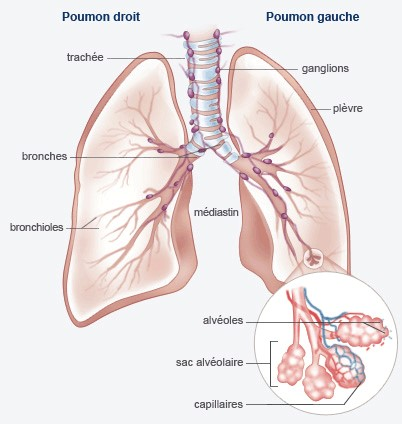
\includegraphics[scale=0.7]{gfx/poumon.jpg} 
\captionof{figure}{Poumon}
       \label{poumon}
\end{center}

		\section{Bronche et Bronchioles}
Les bronches primaires (ou souches) se divisent en bronches lobaires puis en bronches segmentaires pour finir par les bronchioles. D’architecture semblable à la trachée, les bronches primaires présentent un épithélium de type respiratoire identique à celui de la trachée mais aussi quelques différences: une discontinuité des anneaux cartilagineux, elles présentent également un réseau de fibres élastiques plus important dans le chorion qui fait office de séparation avec la sous muqueuse qui contient moins de structures glandulaires.
Les bronchioles sont très fines (0.5 à 1mm de diamètre) divisées en trois types chacun étant progressivement de plus en plus petit : les bronchioles lobaires, les bronchioles terminales et les bronchioles respiratoires. Il n’y a pas d’échange d’air dans les bronchioles lobaire et terminales par contre on a un échange au niveau des bronchioles respiratoire. La fonction primaire des bronchioles est de conduire l’air des bronches aux alvéoles et de contrôler le débit d’air distribué dans le poumon par constriction ou dilatation. La structure des bronchioles est sensiblement différente des celles des bronches. Alors que les bronches sont entourées d’un anneau de cartilage qui permet de les maintenir ouvert, les bronchioles sont-elles entourées d’un mur de muscle lisse permettant de dilater et de contracter les voies respiratoires contrôlant ainsi la livraison d’air aux alvéoles. Leur muqueuse est formée d’un épithélium simple cylindrique dépourvu de cellules caliciformes et pauvre en cellules ciliées. Le chorion est réduit à une fine lame élastique et la sous muqueuse qui se confond avec l’adventice ne contient pas de glandes. (Figure\ref{bronche})
\begin{center}
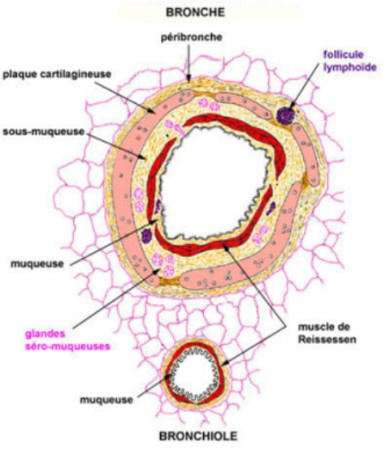
\includegraphics[scale=1.6]{gfx/bronche.jpg} 
\captionof{figure}{Bronche}
       \label{bronche}
\end{center}


		\section{Alvéoles}
A l’aboutissement de l’arbre bronchique on retrouve les alvéoles regroupées en acinus pulmonaire. Un acinus est constitué des 5 à 6 alvéoles entourées d’un réseau de capillaire sanguin fixé et intiment lié à la fonction des alvéoles.
L’épithélium alvéolaire est constitué de pneumocytes de deux types différents type I (membraneux) et type II (granuleux). La barrière alvéolo-capillaire au travers de laquelle est assuré la fonction d’échanges gazeux est formée des Pneumocytes de type I des alvéoles et des cellules endothéliales des capillaires. Alors que la proportion en Pneumocytes I et II est sensiblement identique, les Pneumocytes de type I, du fait de leurs structures fines (0,1 à 0,2\micro\metre d'épaisseur) et étalées, couvrent 95\% de la surface alvéolaire. Ceci a pour conséquence de conférer à l’épithélium alvéolaire une caractéristique souple très étendu qui favorise les échanges gazeux, mais aussi très fragile qui le rend vulnérable aux attaques microbiennes et aux polluants.
Les pneumocytes de type II sont de forme cubique et présente une microvillosité au niveau de leurs pôle apical. Leurs aspect granuleux est dû à leur cytoplasme riche en organites dont un spécifique, les corps lamellaires qui sécrètent le surfactant pulmonaire, de plus ils présentent un réticulum endoplasmique et un appareil de Golgi surdéveloppés signe d’un métabolisme très actif. Le surfactant sécrété (et aussi recyclé), par les corps lamellaires des pneumocytes de type II, a pour fonction de fluidifier le mucus et de facilite les échanges gazeux, de diminuer la tension de surface des alvéoles afin qu'elles ne s'effondrent pas sur elles-mêmes pendant la respiration et à la conservation de l'élasticité des poumons. (Figure \ref{alveol})
\begin{center}
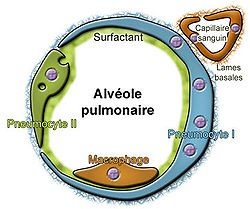
\includegraphics[scale=0.7]{gfx/alveole.jpg} 
\captionof{figure}{Alvéole}
       \label{alveol}
\end{center}

		\section{Pathologies}
Les maladies pulmonaires ont essentiellement des causes infectieuses (bactéries, virus ou champignons pathogènes). Le plus fréquent étant le pneumocoque (Streptococcus pneumoniae) qui est aussi l’un des plus dangereux. Parmi les pathologies pulmonaires fréquentes on trouve l’asthme, les bronchopneumopathies chroniques obstructives (BCPO) caractérisé par un rétrécissement irréversible des bronches, cancers et la mucoviscidose maladie génétique caractérisé par une production importante d’un mucus épais qui entraîne d’important troubles respiratoires. On peut en citer pleins d’autre mais c’est sur cette dernière pathologie que notre étude se concentre.




%------------------------------------------------

% \subsection{Subsection Title}

% Content % Chapter 2
% Chapter X

\chapter{CHAPTER} % Chapter title


\label{ch:01-03} % For referencing the chapter elsewhere, use \autoref{ch:name} 

%----------------------------------------------------------------------------------------

% \section{}

Content

%------------------------------------------------

% \subsection{Subsection Title}

% Content % Chapter 3
% Chapter X

\chapter{CHAPTER} % Chapter title


\label{ch:01-04} % For referencing the chapter elsewhere, use \autoref{ch:name} 

%----------------------------------------------------------------------------------------

% \section{}

Content

%------------------------------------------------

% \subsection{Subsection Title}

% Content % Chapter 4 

% \cleardoublepage % Empty page before the start of the next part

%------------------------------------------------

\ctparttext{\blindtext} % Text on the Part 2 page describing the content in Part 2
% Soulever dans ce § les principales questions soulevées dans cette partie

\part{PART II} % Second part of the thesis

% Chapter X

\chapter{CHAPTER} % Chapter title


\label{ch:02-01} % For referencing the chapter elsewhere, use \autoref{ch:name} 

%----------------------------------------------------------------------------------------

% \section{}

Content

%------------------------------------------------

% \subsection{Subsection Title}

% Content % Chapter 1
% Chapter X

\chapter{CHAPTER} % Chapter title


\label{ch:02-02} % For referencing the chapter elsewhere, use \autoref{ch:name} 

%----------------------------------------------------------------------------------------

% \section{}

Content

%------------------------------------------------

% \subsection{Subsection Title}

% Content % Chapter 2
% Chapter X

\chapter{CHAPTER} % Chapter title


\label{ch:02-03} % For referencing the chapter elsewhere, use \autoref{ch:name} 

%----------------------------------------------------------------------------------------

% \section{}

Content

%------------------------------------------------

% \subsection{Subsection Title}

% Content % Chapter 3
% Chapter X

\chapter{CHAPTER} % Chapter title


\label{ch:02-04} % For referencing the chapter elsewhere, use \autoref{ch:name} 

%----------------------------------------------------------------------------------------

% \section{}

Content

%------------------------------------------------

% \subsection{Subsection Title}

% Content % Chapter 4

\cleardoublepage % Empty page before the start of the next part


% %------------------------------------------------

\ctparttext{\blindtext} % Text on the Part 3 page describing the content in Part 3

\part{PART III} % Third part of the thesis

% Chapter X

\chapter{CHAPTER} % Chapter title


\label{ch:03-01} % For referencing the chapter elsewhere, use \autoref{ch:name} 

%----------------------------------------------------------------------------------------

% \section{}

Content

%------------------------------------------------

% \subsection{Subsection Title}

% Content % Chapter 1
% Chapter X

\chapter{CHAPTER} % Chapter title


\label{ch:03-02} % For referencing the chapter elsewhere, use \autoref{ch:name} 

%----------------------------------------------------------------------------------------

% \section{}

Content

%------------------------------------------------

% \subsection{Subsection Title}

% Content % Chapter 2
% Chapter X

\chapter{CHAPTER} % Chapter title


\label{ch:03-03} % For referencing the chapter elsewhere, use \autoref{ch:name} 

%----------------------------------------------------------------------------------------

% \section{}

Content

%------------------------------------------------

% \subsection{Subsection Title}

% Content % Chapter 3
% % Chapter X

\chapter{CHAPTER} % Chapter title


\label{ch:03-04} % For referencing the chapter elsewhere, use \autoref{ch:name} 

%----------------------------------------------------------------------------------------

% \section{}

Content

%------------------------------------------------

% \subsection{Subsection Title}

% Content % Chapter 4     Discussions ???
% Chapter X

\chapter{CHAPTER} % Chapter title


\label{ch:03-05} % For referencing the chapter elsewhere, use \autoref{ch:name} 

%----------------------------------------------------------------------------------------

% \section{}

Content

%------------------------------------------------

% \subsection{Subsection Title}

% Content % Chapter 5


% %------------------------------------------------

\ctparttext{\blindtext} % Text on the Part 3 page describing the content in Part 3

\part{PART IV} % Third part of the thesis

% Chapter X

\chapter{CHAPTER} % Chapter title


\label{ch:04-01} % For referencing the chapter elsewhere, use \autoref{ch:name} 

%----------------------------------------------------------------------------------------

% \section{}

Content

%------------------------------------------------

% \subsection{Subsection Title}

% Content % Chapter 1
% Chapter X

\chapter{CHAPTER} % Chapter title


\label{ch:04-02} % For referencing the chapter elsewhere, use \autoref{ch:name} 

%----------------------------------------------------------------------------------------

% \section{}

Content

%------------------------------------------------

% \subsection{Subsection Title}

% Content % Chapter 2
% Chapter X

\chapter{CHAPTER} % Chapter title


\label{ch:04-03} % For referencing the chapter elsewhere, use \autoref{ch:name} 

%----------------------------------------------------------------------------------------

% \section{}

Content

%------------------------------------------------

% \subsection{Subsection Title}

% Content % Chapter 3
% % Chapter X

\chapter{CHAPTER} % Chapter title


\label{ch:04-04} % For referencing the chapter elsewhere, use \autoref{ch:name} 

%----------------------------------------------------------------------------------------

% \section{}

Content

%------------------------------------------------

% \subsection{Subsection Title}

% Content % Chapter 4      Discussions ???
% Chapter X

\chapter{CHAPTER} % Chapter title


\label{ch:04-05} % For referencing the chapter elsewhere, use \autoref{ch:name} 

%----------------------------------------------------------------------------------------

% \section{}

Content

%------------------------------------------------

% \subsection{Subsection Title}

% Content % Chapter 5

% \cleardoublepage % Empty page before the start of the next part

\part{PART V} % Third part of the thesis
% Chapter X

\chapter{CHAPTER} % Chapter title


\label{ch:05-01} % For referencing the chapter elsewhere, use \autoref{ch:name} 

%----------------------------------------------------------------------------------------

% \section{}

Content

%------------------------------------------------

% \subsection{Subsection Title}

% Content % Chapter 5


%----------------------------------------------------------------------------------------
%	THESIS CONTENT - APPENDICES
%----------------------------------------------------------------------------------------

\appendix
\addtocontents{toc}{\protect\vspace{1em}}

% \part{Annexes} % New part of the thesis for the appendix

% % \cleardoublepage

%----------------------------------------------------------------------------------------
%	POST-CONTENT THESIS PAGES
%----------------------------------------------------------------------------------------

% \listoffigures
% \cleardoublepage

% \listoftables
% \cleardoublepage

%----------------------------------------------------------------------------------------
%	Glossary
%----------------------------------------------------------------------------------------
\newpage
\refstepcounter{dummy}

\setglossarystyle{altlist} 
\printglossary[title={Glossaire}]

% Bibliography
% %\renewcommand*{\bibname}{new name} % Uncomment to change the name of the bibliography
% %\setbibpreamble{} % Uncomment to include a preamble to the bibliography - some text before the reference list starts

{%
\setstretch{1.1}
\renewcommand{\bibfont}{\normalfont\small}
\setlength{\biblabelsep}{0pt}
\setlength{\bibitemsep}{0.5\baselineskip plus 0.5\baselineskip}
\printbibliography[nottype=online]
% \printbibliography[heading=subbibliography,title={Webpages},type=online,prefixnumbers={@}]
}
\cleardoublepage

% \cleardoublepage% Publications - a page listing research articles written using content in the thesis

\pdfbookmark[1]{Publications}{Publications} % Bookmark name visible in a PDF viewer

\chapter*{Publications} % Publications page text

Some ideas and figures have appeared previously in the following publications:

\noindent Put your publications from the thesis here. The packages \texttt{multibib} or \texttt{bibtopic} etc. can be used to handle multiple different bibliographies in your document.

%\begin{refsection}[ownpubs]
%    \small
%    \nocite{*} % is local to to the enclosing refsection
%    \printbibliography[heading=none]
%\end{refsection}

%\emph{Attention}: This requires a separate run of \texttt{bibtex} for your \texttt{refsection}, \eg, \texttt{ClassicThesis1-blx} for this file. You might also use \texttt{biber} as the backend for \texttt{biblatex}. See also \url{http://tex.stackexchange.com/questions/128196/problem-with-refsection}. % Publications from the thesis page

% % Colophon (a brief description of publication or production notes relevant to the edition)
% !TEX root = ../my-thesis.tex
%
\pagestyle{empty}
\hfill
\vfill
\pdfbookmark[0]{Colophon}{Colophon}
\section*{Colophon}

This thesis was typeset with \LaTeXe.
It uses the \textit{Clean Thesis} style developed by Ricardo Langner.
The design of the \textit{Clean Thesis} style is inspired by user guide documents from Apple Inc.

Download the \textit{Clean Thesis} style at \url{http://cleanthesis.der-ric.de/}.
% \cleardoublepage

% !TEX root = ../my-thesis.tex
%
%************************************************
% Declaration
%************************************************
\pdfbookmark[0]{Declaration}{Declaration}
\chapter*{Declaration}
\label{sec:declaration}
\thispagestyle{empty}

You can put your declaration here, to declare that you have completed your work solely and only with the help of the references you mentioned.

\bigskip

\noindent\textit{\thesisUniversityCity, \thesisDate}

\smallskip

\begin{flushright}
	\begin{minipage}{5cm}
		\rule{\textwidth}{1pt}
		\centering\thesisName
	\end{minipage}
\end{flushright}

%*****************************************
%*****************************************
% \clearpage
\mbox{}

%----------------------------------------------------------------------------------------

% **************************************************
% End of Document CONTENT
% **************************************************
\end{document}
